\documentclass[english]{article}
\usepackage[utf8x]{inputenc}
\usepackage[T1]{fontenc}
\usepackage{babel}
\usepackage{amsmath}
\usepackage{graphicx}
\usepackage{hyperref}
\usepackage{fancyhdr}

\graphicspath{{../images/}}
\pagestyle{fancy}
\fancyhf{}
\renewcommand{\headrulewidth}{0pt}
\setlength{\headheight}{40pt} 
\usepackage[a4paper,top=2cm,bottom=2cm,left=3cm,right=3cm,marginparwidth=1.75cm]{geometry}

\begin{document}

%-------------------------------------------------------%

\title{\bf Designing Sustainable Agriculture Databases: Relational and Document-Based Approaches}
\author{Josh Le Grice - 720017170}
\date{}
\maketitle
\thispagestyle{fancy}


%-------------------------------------------------------%
\section{Introduction}
Introduce the need for this database and why it is helpful for agricultural businesses.

%-------------------------------------------------------%
\section{Database Design}

Define the tables needed.
- Farm
- Crops
- Soils
- Resources
- Sustainability Initiatives

\begin{figure}[h!]
\centering
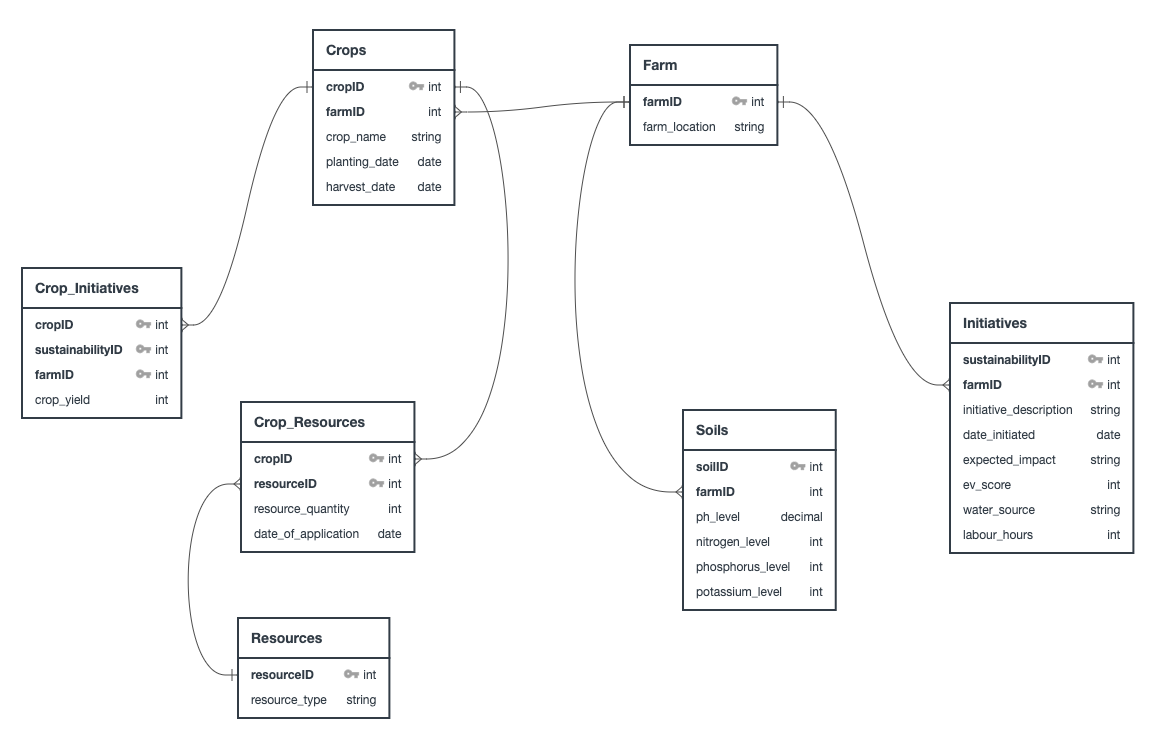
\includegraphics[width=\textwidth]{DatabaseDiagram}
\caption{Entity Relationship Diagram of the Agriculture Database}
\end{figure}

%-------------------------------------------------------%
\section{SQL Implementation}

Talk about how it is implemented in SQL

%-------------------------------------------------------%
\section{RESTful API Design}

How the API is created, the commands needed and what tehy will get
Also, include link to the working app

%-------------------------------------------------------%
\section{Document Based Design Implmentation}

Evaluate the limitaions of the Relational design and propose the document based approach using mongodb, could implement if have time.

%-------------------------------------------------------%
\section{Conclusions}

Summarise key takeways

%-------------------------------------------------------%
% Figures and tables
\clearpage

%-------------------------------------------------------%
\clearpage
% Include your references here.
\bibliographystyle{plain}
\bibliography{references}

%-------------------------------------------------------%

%-------------------------------------------------------%
\clearpage
% Include your appendix here, if necessary.
% \section*{Appendix}
% % Appendix (optional, unlimited)
% % Code snippets, supplementary figures, tables, or additional materials.
% % Will not be marked but can provide supporting evidence.

%-------------------------------------------------------%
\end{document}
